\section{Messgleichrichter}\label{sec:3}

\subsection{Aufgabenstellung}

Es wird eine Messgleichrichterschaltung am Messverstärkerbrett aufgebaut und das dynamische sowie das statische Verhalten untersucht.

\subsection{Versuchsaufbau}


\begin{figure}[h]
	\centering
	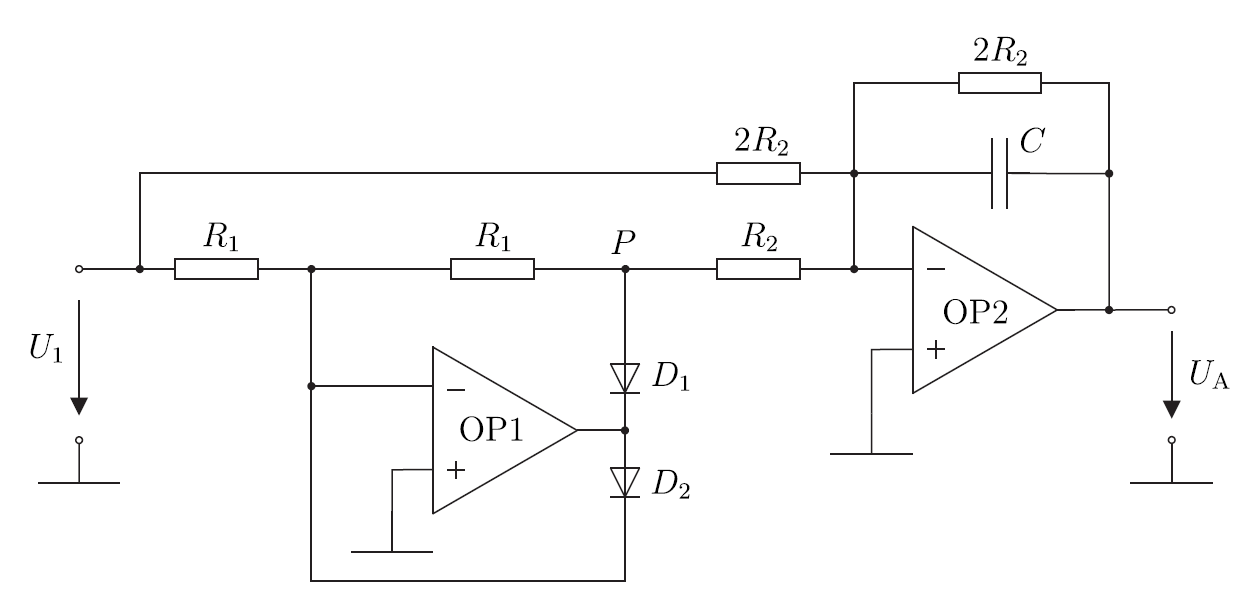
\includegraphics[width=0.7\textwidth]{images/30_Schaltung.png}
	\caption{Messgleichrichterschaltung}\label{fig:30_schaltung}
\end{figure}

Für den Aufbau wurden die Verfügbaren Komponenten am Messverstärkerbrett verwendet. Die Schaltung ist in Abbildung \ref{fig:30_schaltung} dargestellt. Für den Widerstand wurde $R=\SI{1}{\kilo\ohm}$ gewählt und für den optionalen Kondensator $C=\SI{1}{\mu\farad}$, um eine sichtbare Glättung des Ausgangssignals zu erreichen. Das Eingangssignal $U_1$ wird mit einem Funktionsgenerator erzeugt und auf Kanal 1 des Oszilloskops gegeben. Der Ausgang $U_\mathrm{A}$ der Schaltung wird mit Kanal 2 des Oszilloskops betrachtet.

\subsubsection{Funktionsweise}

Die Funktion der Schaltung ist zum einen, den Betrag des Eingangssignals zu bilden.

Ein Umkehrsummierer bildet die negative Summe der Eingangsspannung $U_1$ und der Spannung an Punkt $P$ in \autoref{fig:30_schaltung}. Dabei ist der Widerstand $R_2$ am Punkt $P$ halb so groß wie die Restliche Beschaltung mit $2R_2$ des Umkehrsummierers, sodass durch den größeren Strom diese Spannung doppelt gewichtet wird. (Vergleiche \cite[S.~80. Gl.~4.1]{EMTPraktikum2025})
\begin{equation}
U_\mathrm{A} = -\left(\frac{2R_2}{2R_2}U_1 + \frac{2R_2}{R_2}U_P\right) = -\left(U_1 + 2U_P\right) = \lvert U_1\rvert\label{eq:30_betrag}
\end{equation}
OP 1 dient als invertierender Verstärker. Die Dioden verursachen eine Fallunterscheidung.
\begin{itemize}[noitemsep]
	\item Ist $U_1 < 0$, so leitet $D_2$ und $D_1$ sperrt. Dadurch liegt Punkt $P$ auf \SI{0}{\volt}.
	\item Ist $U_1 > 0$, so leitet $D_1$ und $D_2$ sperrt. Dadurch liegt Punkt $P$ auf $-U_1$.
\end{itemize}
Einsetzen in \autoref{eq:30_betrag} liefert somit in beiden Fällen den Betrag des Eingangssignals.

Fügt man den optionalen Kondensator $C$ hinzu, so wird zusätzlich eine Glättung des Ausgangssignals erreicht. Der Gleichspannungswert beträgt dann den Gleichrichtwert des Betrags des Eingangssignals \cite[S.~18, Gl.~1.26]{EMTPraktikum2025}.
\[
U_A = \overline{\lvert U_1 \rvert} = \frac{1}{T}\int_{0}^{T} \lvert U_1(t) \rvert \mathrm{d}t
\]



\subsection{Statische Betrachtung}

\subsubsection{Einstellungen}

Für die Statische Betrachtung wird ein niederfrequentes rechtecksignal mit einer Amplitude von $U_{1,\mathrm{pp}}=\SI{10}{\volt}$ und einer Frequenz von $f=\SI{5}{\hertz}$ eingestellt. Der Kondensator wird jeweils mit Bananensteckern hinzu- oder abgesteckt.

\subsubsection{Messergebnisse}


Ohne Kondensator ist die Form der Schwankung gleich des Rechtecksignals.
Mit kondensator ist an den Sprüngen des Rechtechs eine Lade- bzw. Entladekurve zu erkennen.

\begin{figure}[h]
	\begin{minipage}[t]{.5\textwidth}
		\centering	
		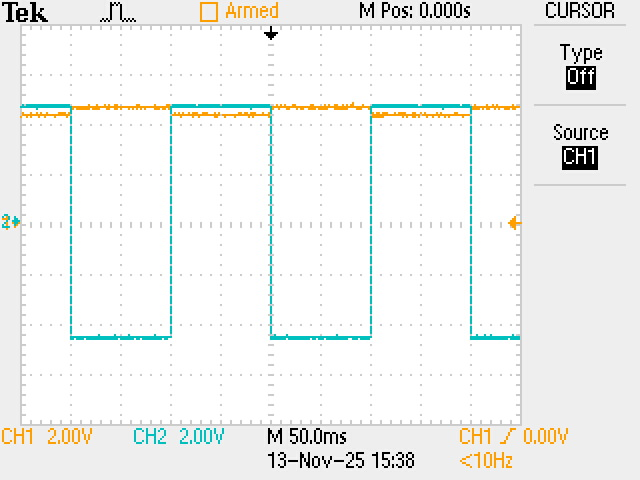
\includegraphics[width=.8\textwidth]{images/oszi/30_MGL_Statisch_ohne_C.JPG}\\
		(a) ohne C\label{fig:30_mgl_statisch_ohne_c}
	\end{minipage}\hfill
	\begin{minipage}[t]{.5\textwidth}
		\centering	
		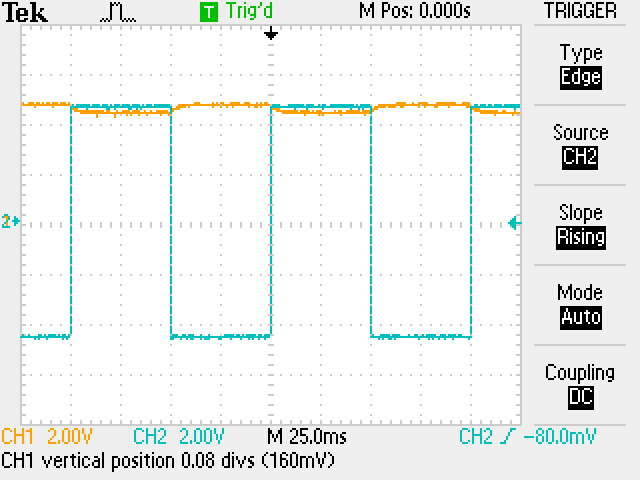
\includegraphics[width=.8\textwidth]{images/oszi/30_MGL_Statisch_mit_C.JPG}\\
		(b) mit C\label{fig:30_mgl_statisch_mit_c}
	\end{minipage}
	\caption{Statische Betrachtung des Messgleichrichters}\label{fig:30_statisch}
\end{figure}

\newpage

\subsection{Dynamische Betrachtung}

\subsubsection{Einstellungen}

Für die Statische Betrachtung wird ein sinusförmiges Signal mit einer Amplitude von $U_{1,\mathrm{pp}}=\SI{10}{\volt}$ und verschiedenen Frequenzen eingestellt: \SI{10}{\hertz}, \SI{100}{\hertz} und \SI{1}{\kilo\hertz}. Der Kondensator wird jeweils mit Bananensteckern hinzu- oder abgesteckt

\subsubsection{Messergebnisse}

Ohne dem Kondensator:

\begin{figure}[h]
	\begin{minipage}[t]{.32\textwidth}
		\centering	
		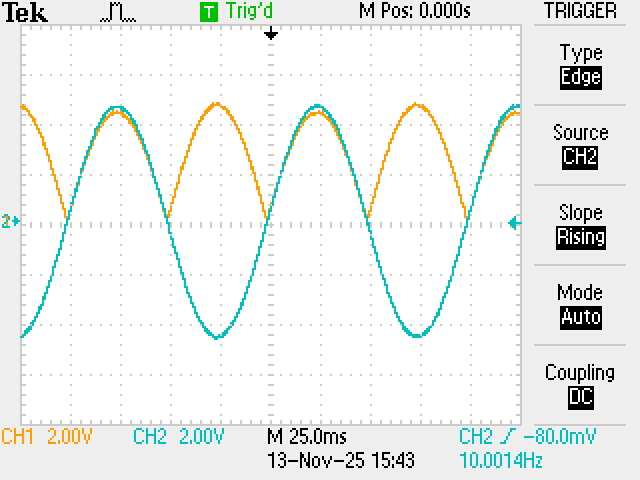
\includegraphics[width=.9\textwidth]{images/oszi/30_MGL_Dyn_ohne_C_10Hz.JPG}\\
		(a) bei \SI{10}{\hertz} ohne C
	\end{minipage}\hfill
	\begin{minipage}[t]{.32\textwidth}
		\centering	
		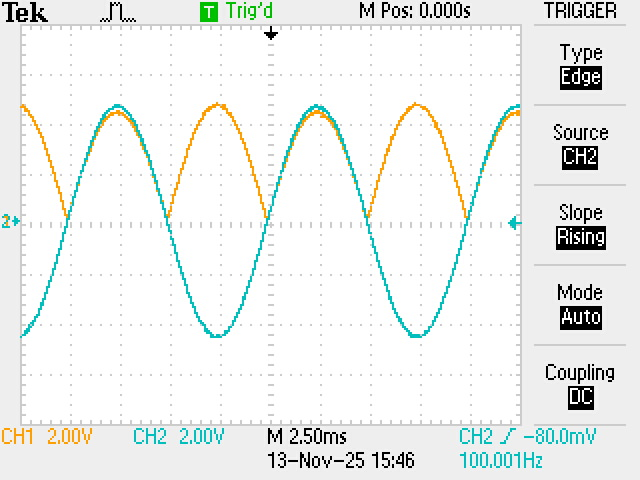
\includegraphics[width=.9\textwidth]{images/oszi/30_MGL_Dyn_ohne_C_100Hz.JPG}\\
		(b) bei \SI{100}{\hertz} ohne C
	\end{minipage}\hfill
	\begin{minipage}[t]{.32\textwidth}
		\centering	
		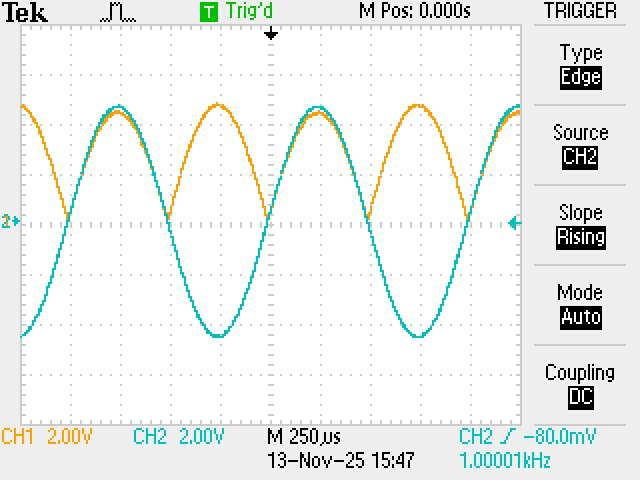
\includegraphics[width=.9\textwidth]{images/oszi/30_MGL_Dyn_ohne_C_1kHz.JPG}\\
		(c) bei \SI{1}{\kilo\hertz} ohne C
	\end{minipage}
	\caption{Dynamische Betrachtung des Messgleichrichters ohne Kondensator bei verschiedenen Frequenzen}\label{fig:30_dyn_ohne_c}
\end{figure}

Mit dem Kondensator:

\begin{figure}[h]
	\begin{minipage}[t]{.32\textwidth}
		\centering	
		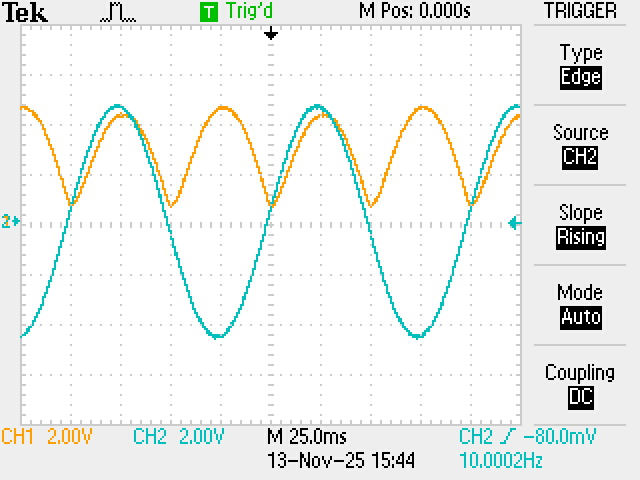
\includegraphics[width=.9\textwidth]{images/oszi/30_MGL_Dyn_mit_C_10Hz.JPG}\\
		(a) bei \SI{10}{\hertz} mit C
	\end{minipage}\hfill
	\begin{minipage}[t]{.32\textwidth}
		\centering	
		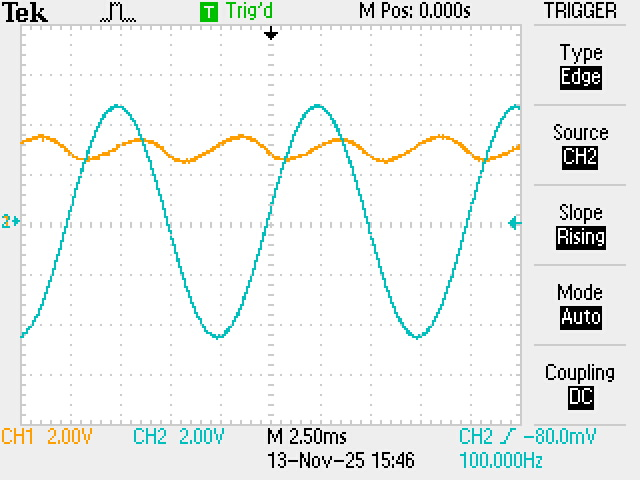
\includegraphics[width=.9\textwidth]{images/oszi/30_MGL_Dyn_mit_C_100Hz.JPG}\\
		(b) bei \SI{100}{\hertz} mit C
	\end{minipage}\hfill
	\begin{minipage}[t]{.32\textwidth}
		\centering	
		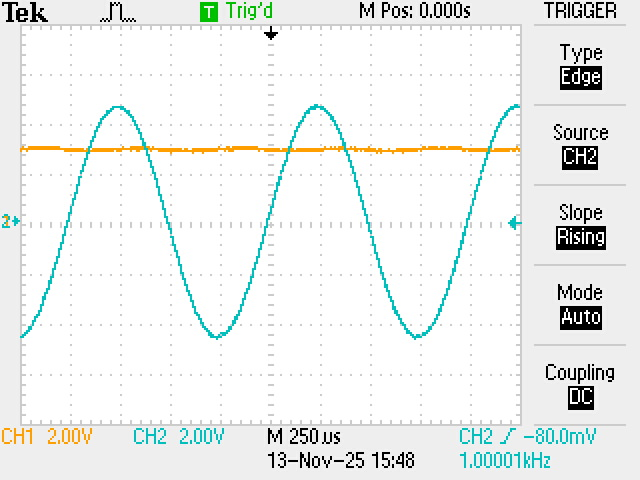
\includegraphics[width=.9\textwidth]{images/oszi/30_MGL_Dyn_mit_C_1kHz.JPG}\\
		(c) bei \SI{1}{\kilo\hertz} mit C
	\end{minipage}
	\caption{Dynamische Betrachtung des Messgleichrichters mit Kondensator bei verschiedenen Frequenzen}\label{fig:30_dyn_mit_c}
\end{figure}

\subsection{Erkenntnisse}

\paragraph{Statisches Verhalten} Idealerweise sollte bei der Gleichrichtung des Rechtecks eine konstante Gleichspannung am Ausgang anliegen. In Abbildung \ref{fig:30_statisch} ist zu sehen, dass das Signal nahe der Amplitude etwa um $0.2 \mathrm{RE} = \SI{0.4}{\volt}$ schwankt. Dies ist womöglich auf Bauteiltoleranzen der Widerstände und der Ungleichmäßigen erwärmung der Dioden zurückzuführen.

\paragraph{Dynamisches Verhalten} Ohne Kondensator wird die negative Halbwelle nach obengeklappt, wodurch die Betragbildung gesehen werden kann. Mit Kondensator wird das Ausgangssignal geglättet, wobei die Glättung bei höheren Frequenzen besser funktioniert als bei niedrigen Frequenzen, da der Kondensator mehr Zeit hat sich zu entladen. Um dem entgegen zu wirken, kann auch die Kapazität des Kondensators erhöht werden, wodurch jedoch das Umladen im falle einer Änderung der Eingangsamplitude länger dauert.